% Options for packages loaded elsewhere
\PassOptionsToPackage{unicode}{hyperref}
\PassOptionsToPackage{hyphens}{url}
%
\documentclass[
]{article}
\usepackage{amsmath,amssymb}
\usepackage{lmodern}
\usepackage{iftex}
\ifPDFTeX
  \usepackage[T1]{fontenc}
  \usepackage[utf8]{inputenc}
  \usepackage{textcomp} % provide euro and other symbols
\else % if luatex or xetex
  \usepackage{unicode-math}
  \defaultfontfeatures{Scale=MatchLowercase}
  \defaultfontfeatures[\rmfamily]{Ligatures=TeX,Scale=1}
\fi
% Use upquote if available, for straight quotes in verbatim environments
\IfFileExists{upquote.sty}{\usepackage{upquote}}{}
\IfFileExists{microtype.sty}{% use microtype if available
  \usepackage[]{microtype}
  \UseMicrotypeSet[protrusion]{basicmath} % disable protrusion for tt fonts
}{}
\makeatletter
\@ifundefined{KOMAClassName}{% if non-KOMA class
  \IfFileExists{parskip.sty}{%
    \usepackage{parskip}
  }{% else
    \setlength{\parindent}{0pt}
    \setlength{\parskip}{6pt plus 2pt minus 1pt}}
}{% if KOMA class
  \KOMAoptions{parskip=half}}
\makeatother
\usepackage{xcolor}
\usepackage[margin =2cm]{geometry}
\usepackage{listings}
\newcommand{\passthrough}[1]{#1}
\lstset{defaultdialect=[5.3]Lua}
\lstset{defaultdialect=[x86masm]Assembler}
\usepackage{graphicx}
\makeatletter
\def\maxwidth{\ifdim\Gin@nat@width>\linewidth\linewidth\else\Gin@nat@width\fi}
\def\maxheight{\ifdim\Gin@nat@height>\textheight\textheight\else\Gin@nat@height\fi}
\makeatother
% Scale images if necessary, so that they will not overflow the page
% margins by default, and it is still possible to overwrite the defaults
% using explicit options in \includegraphics[width, height, ...]{}
\setkeys{Gin}{width=\maxwidth,height=\maxheight,keepaspectratio}
% Set default figure placement to htbp
\makeatletter
\def\fps@figure{htbp}
\makeatother
\setlength{\emergencystretch}{3em} % prevent overfull lines
\providecommand{\tightlist}{%
  \setlength{\itemsep}{0pt}\setlength{\parskip}{0pt}}
\setcounter{secnumdepth}{-\maxdimen} % remove section numbering
\usepackage{titlesec}
\titleformat{\paragraph}
   {\normalfont\bfseries}
   {}
   {0pt}
   {}
\lstset{
  breaklines=TRUE
}

\usepackage[T1]{fontenc}
\usepackage{babel}
\usepackage{geometry}
\usepackage{titling}
\usepackage{blindtext}

\setlength{\droptitle}{-4em}     % Eliminate the default vertical space
\addtolength{\droptitle}{-4pt}   % Only a guess. Use this for adjustment
\pretitle{\begin{center} \vspace{10cm}}
\ifLuaTeX
  \usepackage{selnolig}  % disable illegal ligatures
\fi
\IfFileExists{bookmark.sty}{\usepackage{bookmark}}{\usepackage{hyperref}}
\IfFileExists{xurl.sty}{\usepackage{xurl}}{} % add URL line breaks if available
\urlstyle{same} % disable monospaced font for URLs
\hypersetup{
  pdftitle={Different Types of Regression},
  pdfauthor={B.M Njuguna},
  hidelinks,
  pdfcreator={LaTeX via pandoc}}

\title{\textbf{Different Types of Regression}}
\author{\textbf{B.M Njuguna}}
\date{\textbf{2022-09-09}}

\begin{document}
\maketitle

\newpage 
\tableofcontents
\newpage

\hypertarget{regression-analysis}{%
\section{1.0 Regression Analysis}\label{regression-analysis}}

Regression analysis is a set of statistical methods used to identify or
estimate the relationship(s) between the \textbf{dependent} and
\textbf{independent} variable(s). It can also be utilized to assess the
strength of the relationship and also to model the future relationship
between the variables. The dependent variable which is also known as
\textbf{response variable} is the variable being tested or measured in
an experiment, while the independent or the \textbf{explanatory or
predictor variable} is the variable which is included to the model to
explain changes in the dependent variable. In most cases, the dependent
variable is denoted by \(y\) while the independent variable is usually
denoted by \(x\).

\hypertarget{types-of-regression-analysis}{%
\subsection{1.1 Types of Regression
Analysis}\label{types-of-regression-analysis}}

There are several types of regression analysis depending on what you
want to achieve, or depending on the nature of the study or the nature
of the variables. They include;\footnote{ This paper was compiled by
  Brian Mwangi Njuguna on 22-08-2022, for acadameic purposes}

\begin{enumerate}
\def\labelenumi{\arabic{enumi}.}
\item
  Linear Regression
\item
  Logistic Regression
\item
  Polynomial Regression
\item
  Ridge Regression
\item
  Quantile Regression
\item
  Bayesian Linear Regression
\item
  Principal Component Regression
\item
  Partial Least Square Regression amongst other types.
\end{enumerate}

\newpage

\hypertarget{linear-regression}{%
\section{2.0 Linear Regression}\label{linear-regression}}

A linear regression is a regression model that estimates the
relationship between the dependent and the independent variables using a
straight line. A linear regression model is as follows;

\[y_i=\beta_0+\beta_1x_{i1}+\beta_2x_{i2}+{...}+\beta_px_{ip}+\epsilon_i\]

Where

\begin{itemize}
\item
  \(y_i\) is the response variable.
\item
  \(\beta_k\) is the \(k^{th}\) coefficient, where \(\beta_0\) is the
  constant term in the model.
\item
  \(X_{ij}\) is the \(i^{th}\) observation on the \(j^{th}\) predictor
  variable, \(j = 1, ..., p.\)
\item
  \(\epsilon_i\) is the \(i^{th}\) noise term, that is, random error.
\end{itemize}

If the model includes one predictor variable, that is p=1, then the
model is known as a simple linear regression model.

\hypertarget{simple-linear-regression-model}{%
\subsection{2.1 Simple Linear Regression
model}\label{simple-linear-regression-model}}

A simple linear regression model is of the form;

\[y=\beta_o+\beta_1x\]

where;

\(y\) - is the response variable

\(\beta_0\) - is the intercept. It refers to the value of \(y\) when
\(x=0\).

\(\beta_1\) - is the regression coefficient or the slope. It represents
the change in variable \(y\) caused by a unit change in the explanatory
variable \(x\).

It is used to model the relationship between two continuous variables.
The assumptions are;

\begin{enumerate}
\def\labelenumi{\arabic{enumi}.}
\item
  Linearity- The variables \(x\) and \(y\) must have a linear
  relationship
\item
  The error terms \(\epsilon_i\) are independent and that the error is
  normally distributed with mean 0 and variance \(\sigma^2\). That is;
  \(\epsilon_i\sim N(0,\sigma^2)\)
\end{enumerate}

For example, We may wish to determine whether advertisement and sales
have a linear relationship. Below is a data set containing the budget of
advertisement in various platforms including TV,Radios and Newspaper as
well as the sales, in 1000\$.

\begin{lstlisting}[language=R]
> ## Importing the data set from my library
> setwd("D:/Documents/R-Studio Programms/Regression/Linear Regression")
> library(readxl)
> AdvertisingBudgetandSales <- read_excel("AdvertisingBudgetandSales.xlsx", col_types = c("skip",
+     "numeric", "numeric", "numeric", "numeric"))
> ## view first rows of the data set
> head(AdvertisingBudgetandSales)
\end{lstlisting}

\begin{lstlisting}
## # A tibble: 6 x 4
##   `TV Ad Budget ($)` `Radio Ad Budget ($)` `Newspaper Ad Budget ($)` `Sales ($)`
##                <dbl>                 <dbl>                     <dbl>       <dbl>
## 1              230.                   37.8                      69.2        22.1
## 2               44.5                  39.3                      45.1        10.4
## 3               17.2                  45.9                      69.3         9.3
## 4              152.                   41.3                      58.5        18.5
## 5              181.                   10.8                      58.4        12.9
## 6                8.7                  48.9                      75           7.2
\end{lstlisting}

I am going to fit a simple linear regression model where sales is my
response variable and advertisement budget in TV is my predictor
variable. In r, we use the function \emph{lm()} to fit simple linear
regression model as follows;

\begin{lstlisting}[language=R]
> ## slr implying simple linear regression
> slrTV <- lm(formula = `Sales ($)` ~ `TV Ad Budget ($)`, data = AdvertisingBudgetandSales)
> slrTV
\end{lstlisting}

\begin{lstlisting}
## 
## Call:
## lm(formula = `Sales ($)` ~ `TV Ad Budget ($)`, data = AdvertisingBudgetandSales)
## 
## Coefficients:
##        (Intercept)  `TV Ad Budget ($)`  
##            7.03259             0.04754
\end{lstlisting}

From the results above, the model can be written as;
\[\hat{y}=7.03259+0.04754\hat{x}\] or specifically;
\[sales=7.03259+0.04754TVAdvert\] This implies that if there is no
budget on TV advertisement, then the sales will stand at \$7032.59, that
is (7.03259\emph{1000, since the cost or sales were in 1000 dollars).
Then a} \(\hat{\beta_1}\) of 0.04754 implies that for a TV advertisement
budget equal to 1000 dollars, we expect an increase of 47.54 (
0.047541000) units in sales. This implies that;

\[sales=7.03259 +0.04754*1000 =54.57259\space units\]

Since we are operating in units of thousand dollars, this represents a
total sale of 54572.59 dollars. The fitted regression line is shown
below;

\begin{lstlisting}[language=R]
> library(ggplot2)
> PLOT1 <- ggplot(data = AdvertisingBudgetandSales, aes(`TV Ad Budget ($)`, `Sales ($)`)) +
+     geom_point() + stat_smooth(method = lm, se = FALSE)
> 
> PLOT1
\end{lstlisting}

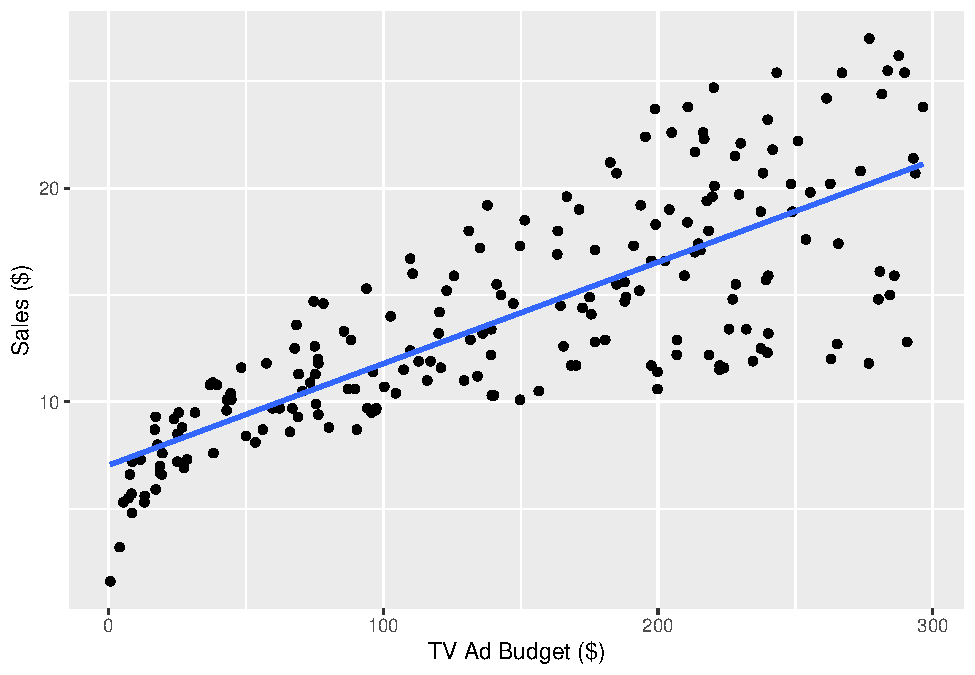
\includegraphics{Types-of-Regressions_files/figure-latex/unnamed-chunk-3-1.pdf}

\hypertarget{model-assessment}{%
\subsubsection{\texorpdfstring{2.1.1 Model
Assessment}{2.1.1 Model Assessment }}\label{model-assessment}}

Before using the model to predict future values, we need to check
whether;

\begin{enumerate}
\def\labelenumi{\arabic{enumi}.}
\item
  There is a statistically significant relationship between the
  predictor variable (TV advert) and the response variable (sales)
\item
  The model fits well with the data.
\end{enumerate}

Using the \emph{summary()} function, we will get more insight about the
model.

\begin{lstlisting}[language=R]
> summary(slrTV)
\end{lstlisting}

\begin{lstlisting}
## 
## Call:
## lm(formula = `Sales ($)` ~ `TV Ad Budget ($)`, data = AdvertisingBudgetandSales)
## 
## Residuals:
##     Min      1Q  Median      3Q     Max 
## -8.3860 -1.9545 -0.1913  2.0671  7.2124 
## 
## Coefficients:
##                    Estimate Std. Error t value Pr(>|t|)    
## (Intercept)        7.032594   0.457843   15.36   <2e-16 ***
## `TV Ad Budget ($)` 0.047537   0.002691   17.67   <2e-16 ***
## ---
## Signif. codes:  0 '***' 0.001 '**' 0.01 '*' 0.05 '.' 0.1 ' ' 1
## 
## Residual standard error: 3.259 on 198 degrees of freedom
## Multiple R-squared:  0.6119, Adjusted R-squared:  0.6099 
## F-statistic: 312.1 on 1 and 198 DF,  p-value: < 2.2e-16
\end{lstlisting}

We use the p-value or the t-statistic to check whether there is a
statistically significant relationship between the given predictor
variable and the response variable. That is, we check whether or not the
\(\beta\) coefficient of the predictor variable is significantly
different from zero. The hypothesis is formulated as;

\[H_0:\hat{\beta_1}=0\space\space Vs\space\space \space H_1:\hat{\beta_1\neq 0}\]

In this case, the p-value is less than 0.05(\(\alpha\)) hence we reject
the null hypothesis and conclude that there is a statistically
significant relationship between sales and TV advertisement. We rarely
test \(\hat{\beta_0}\). The t-statistic is calculated as;

\[t=\frac{\hat{\beta_1}-0}{SE(\hat{\beta_1})}\],

where \(SE\) is the standard error of the coefficient \(\hat{\beta_1}\).

It is worthy to note that a high t-statistic and a low p-value indicates
that the specific predictor variable should be retained in the
model,like in our case.

The \textbf{standard error} represented by \emph{Std.Error} in the r
output above, measures the variability or the accuracy of the \(\beta\)
coefficients. The standard error is used to calculate the confidence
interval of the coefficients. For example, a 95\% confidence interval of
\(\hat{\beta_1}\) is calculated as;

\[\hat{\beta_1}\pm2SE(\hat{\beta_1})\]

The lower limit;

\[\hat{\beta_1}-2SE(\hat{\beta_1})\]

\[0.047537-2* 0.002691=0.042155\]

The upper limit;

\[\hat{\beta_1}+2SE(\hat{\beta_1})\]

\[0.047537+2* 0.002691=0.042155=0.052919\]

Therefore, there is a 95\% chance that the interval (0.042155,0.052919)
will contain the true value of \(\hat{\beta_1}\). Alternatively, it can
be done using the \emph{confint()} function in r,

\begin{lstlisting}[language=R]
> confint(slrTV)
\end{lstlisting}

\begin{lstlisting}
##                         2.5 %     97.5 %
## (Intercept)        6.12971927 7.93546783
## `TV Ad Budget ($)` 0.04223072 0.05284256
\end{lstlisting}

\hypertarget{model-accuracy}{%
\subsubsection{2.1.2 Model Accuracy}\label{model-accuracy}}

The overall quality of the linear regression can be assessed using the
following three quantities.

\begin{enumerate}
\def\labelenumi{\arabic{enumi}.}
\item
  RSE (Residual Standard Error, also known as the model sigma) - it is
  the standard deviation of the residuals. It represents the average
  variation of observations points around the regression line. When
  comparing two model, the model with the lower RSE is the better one.
  In this case, the RSE is 3.259 which is relatively low.
\item
  R-Squared (\(R^2\)) - It represents the proportion or variation in the
  data that can be explained by the model, where \(0<R^2<1\), but is
  mostly outlined as a percentage for easier interpretation. The higher
  the \(R^2\), the better the model. In this case, the \(R^2= 0.6119\)
  which is equivalent to 61.19\%, implies that 61.19\% of the total
  variation in sales, is explained by the model. As you add more
  predictor variables, \(R^2\) tend to increase, therefore in multiple
  linear regression, we use the \(adjusted\space R^2\), To check the
  accuracy of the model. In simple linear regression, \(R^2\) is the
  square of the Pearson's correlation coefficient \(r\).
\end{enumerate}

\begin{lstlisting}[language=R]
> cor(AdvertisingBudgetandSales$`TV Ad Budget ($)`, AdvertisingBudgetandSales$`Sales ($)`,
+     method = c("pearson"))
\end{lstlisting}

\begin{lstlisting}
## [1] 0.7822244
\end{lstlisting}

\begin{lstlisting}[language=R]
> 0.7822244^2
\end{lstlisting}

\begin{lstlisting}
## [1] 0.611875
\end{lstlisting}

\begin{enumerate}
\def\labelenumi{\arabic{enumi}.}
\setcounter{enumi}{2}
\tightlist
\item
  The F-statistic gives the overall significance of the model. Notice
  that the F-statistic is used to test the overall significance of the
  model while the t-statistic is used to test the significance of the
  individual predictor variables. However, in simple linear regression,
  it has no much use since we only have one predictor variable. It
  becomes useful while dealing with multiple linear regression. In fact,
  for any simple linear regression model with 1 degree of freedom, the
  F-statistic is approximately equal to the square of the t-statistic(of
  \(\hat{\beta_1}\)).
\end{enumerate}

\begin{lstlisting}[language=R]
> 17.67^2
\end{lstlisting}

\begin{lstlisting}
## [1] 312.2289
\end{lstlisting}

\hypertarget{multiple-linear-regression}{%
\subsubsection{2.2. Multiple Linear
Regression}\label{multiple-linear-regression}}

Multiple linear regression is an extension of simple linear regression,
whereby several predictor variables are used to predict the outcome of
the response variable. Assuming that there are three predictor
variables, the model can be written as;

\[y_i=\beta_0+\beta_1x_1+\beta_2x_2+\beta_3x_3\]

For easier understanding, let's build a model for estimating sales based
on advertisement budged invested on TV, Radio and newspaper. This model
can be written as;

\[sales=\beta_0 +\beta_1TV+\beta_2Radio+\beta_3Newspaper\]

In r,it is done as follows;

\begin{lstlisting}[language=R]
> attach(AdvertisingBudgetandSales)
> ## entering the model;, mlr implying multiple linear regression
> 
> mlr <- lm(`Sales ($)` ~ `TV Ad Budget ($)` + `Radio Ad Budget ($)` + `Newspaper Ad Budget ($)`,
+     data = AdvertisingBudgetandSales)
> mlr
\end{lstlisting}

\begin{lstlisting}
## 
## Call:
## lm(formula = `Sales ($)` ~ `TV Ad Budget ($)` + `Radio Ad Budget ($)` + 
##     `Newspaper Ad Budget ($)`, data = AdvertisingBudgetandSales)
## 
## Coefficients:
##               (Intercept)         `TV Ad Budget ($)`  
##                  2.938889                   0.045765  
##     `Radio Ad Budget ($)`  `Newspaper Ad Budget ($)`  
##                  0.188530                  -0.001037
\end{lstlisting}

Therefore, the model can be written as;

\[sales=2.939+0.046TV+0.189Radio-0.001Newspaper\]

For more analysis of the model, we use the \emph{summary ()} function.

\begin{lstlisting}[language=R]
> summary(mlr)
\end{lstlisting}

\begin{lstlisting}
## 
## Call:
## lm(formula = `Sales ($)` ~ `TV Ad Budget ($)` + `Radio Ad Budget ($)` + 
##     `Newspaper Ad Budget ($)`, data = AdvertisingBudgetandSales)
## 
## Residuals:
##     Min      1Q  Median      3Q     Max 
## -8.8277 -0.8908  0.2418  1.1893  2.8292 
## 
## Coefficients:
##                            Estimate Std. Error t value Pr(>|t|)    
## (Intercept)                2.938889   0.311908   9.422   <2e-16 ***
## `TV Ad Budget ($)`         0.045765   0.001395  32.809   <2e-16 ***
## `Radio Ad Budget ($)`      0.188530   0.008611  21.893   <2e-16 ***
## `Newspaper Ad Budget ($)` -0.001037   0.005871  -0.177     0.86    
## ---
## Signif. codes:  0 '***' 0.001 '**' 0.01 '*' 0.05 '.' 0.1 ' ' 1
## 
## Residual standard error: 1.686 on 196 degrees of freedom
## Multiple R-squared:  0.8972, Adjusted R-squared:  0.8956 
## F-statistic: 570.3 on 3 and 196 DF,  p-value: < 2.2e-16
\end{lstlisting}

For multiple linear regression, the first step is to check whether the
model is significant using the F-statistic or the corresponding p-value.
The hypothesis is formulated as;

\[H_0:\hat{\beta_1}=\hat{\beta_2}=\hat{\beta_3}=0 \space\space Vs \space\space H_1:\hat{\beta_i}\neq0 \space for \space i=1,\cdots ,4\]

That is, at least one coefficient is not equal to zero or it is
significant. In this case the \(p-value =2.2e-16<0.05\), hence we reject
the null hypothesis and conclude that the model is significant.

To test the individual significance of the predictor models, we use the
t-statistic. If a predictor variable is not statistically significant,
then the variable should be dropped.

\begin{lstlisting}[language=R]
> summary(mlr)$coefficients
\end{lstlisting}

\begin{lstlisting}
##                               Estimate  Std. Error    t value     Pr(>|t|)
## (Intercept)                2.938889369 0.311908236  9.4222884 1.267295e-17
## `TV Ad Budget ($)`         0.045764645 0.001394897 32.8086244 1.509960e-81
## `Radio Ad Budget ($)`      0.188530017 0.008611234 21.8934961 1.505339e-54
## `Newspaper Ad Budget ($)` -0.001037493 0.005871010 -0.1767146 8.599151e-01
\end{lstlisting}

From the output above, TV and Radio predictor variables are
statistically significant, but Newspaper is not, since its p-value is
greater than 0.05.

The coefficients are interpreted as follows, for a fixed amount of Radio
and Newspaper advertisement budget, spending an additional \$1000 on TV
advertisement leads to an increase in sales by approximately
0.045764645*1000= 45.76465 sale units on average. For the Radio
advertisement it can be interpreted through the same way. However, for
the Newspaper advertisement, it implies that for a fixed amount of TV
and Radio advertisement budget, changes in the advertisement budget will
not significantly change the sales unit, hence we should remove it from
the model, to increase the adjusted R squared.

\begin{lstlisting}[language=R]
> mlr2 <- lm(`Sales ($)` ~ `TV Ad Budget ($)` + `Radio Ad Budget ($)`, data = AdvertisingBudgetandSales)
> summary(mlr2)
\end{lstlisting}

\begin{lstlisting}
## 
## Call:
## lm(formula = `Sales ($)` ~ `TV Ad Budget ($)` + `Radio Ad Budget ($)`, 
##     data = AdvertisingBudgetandSales)
## 
## Residuals:
##     Min      1Q  Median      3Q     Max 
## -8.7977 -0.8752  0.2422  1.1708  2.8328 
## 
## Coefficients:
##                       Estimate Std. Error t value Pr(>|t|)    
## (Intercept)            2.92110    0.29449   9.919   <2e-16 ***
## `TV Ad Budget ($)`     0.04575    0.00139  32.909   <2e-16 ***
## `Radio Ad Budget ($)`  0.18799    0.00804  23.382   <2e-16 ***
## ---
## Signif. codes:  0 '***' 0.001 '**' 0.01 '*' 0.05 '.' 0.1 ' ' 1
## 
## Residual standard error: 1.681 on 197 degrees of freedom
## Multiple R-squared:  0.8972, Adjusted R-squared:  0.8962 
## F-statistic: 859.6 on 2 and 197 DF,  p-value: < 2.2e-16
\end{lstlisting}

The model can be written as;

\[sales=2.921+0.046TV+0.188Radio\]

The confidence interval is;

\begin{lstlisting}[language=R]
> confint(mlr2)
\end{lstlisting}

\begin{lstlisting}
##                            2.5 %     97.5 %
## (Intercept)           2.34034299 3.50185683
## `TV Ad Budget ($)`    0.04301292 0.04849671
## `Radio Ad Budget ($)` 0.17213877 0.20384969
\end{lstlisting}

In multiple linear regression, \(R^2\) is the correlation between the
observed values of the response variable and the fitted (or predicted)
values of the response variable, hence we use the \(adjusted\space R^2\)
to measure the accuracy of the model. In this case, the
\(adjusted\space R^2 =0.8962\), which implies that 89.62\% of the total
variation in the sales, is explained by the model.

\hypertarget{sums-of-squares}{%
\subsubsection{2.2.1 Sums of Squares}\label{sums-of-squares}}

Sums of Squares in regression is a technique used to determine
dispersion of data points. They are divided into two.

\begin{enumerate}
\def\labelenumi{\arabic{enumi}.}
\tightlist
\item
  Sums of Squares due to Regression (SSR)- It is the sum of the
  differences between the fitted values and the mean of the response
  variable.
\end{enumerate}

\[\sum_{n=1}^n(\hat{y}-\bar{y})^2\]

\begin{enumerate}
\def\labelenumi{\arabic{enumi}.}
\setcounter{enumi}{1}
\tightlist
\item
  Sums of Squares Error (SSE). It is the sum of the differences between
  the observed values and the predicted or fitted values.
\end{enumerate}

Total sums of squares is the sum of error and regression sums of
squares.

\[SST=SSR+SSE \]

Note that, if \(SSR=SSE\), then it implies that the regression model
captures all the observed variability and is perfect.

\begin{enumerate}
\def\labelenumi{\arabic{enumi}.}
\setcounter{enumi}{2}
\tightlist
\item
  Residual Sums of Squares (RSS)- It used to measure the amount of
  variance in a data set that is not explained by a regression model. It
  measures the overall difference between the observed data, and the
  values predicted (or fitted) by the estimation model. The lower the
  value, the better the model \[\sum_{n=1}^ne_i^2\]
\end{enumerate}

In r, we get the above information using the Analysis of Variance
function \emph{anova()} as follows;

\begin{lstlisting}[language=R]
> anova(mlr2)
\end{lstlisting}

\begin{lstlisting}
## Analysis of Variance Table
## 
## Response: Sales ($)
##                        Df Sum Sq Mean Sq F value    Pr(>F)    
## `TV Ad Budget ($)`      1 3314.6  3314.6 1172.50 < 2.2e-16 ***
## `Radio Ad Budget ($)`   1 1545.6  1545.6  546.74 < 2.2e-16 ***
## Residuals             197  556.9     2.8                      
## ---
## Signif. codes:  0 '***' 0.001 '**' 0.01 '*' 0.05 '.' 0.1 ' ' 1
\end{lstlisting}

The package \emph{qpcR} in r also have very important functions that are
useful in regression analysis.

\newpage

\hypertarget{regression-model-diagonistics}{%
\section{3.0 Regression Model
Diagonistics}\label{regression-model-diagonistics}}

After performing regression analysis, it is important to check whether
the model works well for the data in hand. This chapter will explore
different ways to check the accuracy of the model. It is important to
evaluate how well the model fits the data because it helps you check
whether the linear regression assumptions have been met or not. For
instance, linear regression assumes that there is a linear relationship
between the predictor variable and the response variable which might not
be the case. The relationship might be polynomial or logarithmic. In
addition, data might contain outliers or extreme values which may affect
the regression. This is achieved by checking the distribution of the
residual errors. Note that the predicted or the fitted values are the
response variable values that you would expect for the given predictor
variable values, according to the built regression model. From the
scatter plot below, you can see that not all points fall exactly on the
regression line. This means that for a given TV or Radio advertisement
budget, the observed or the measured values can be different from the
predicted or fitted values. The difference is known as \textbf{residual
errors}, represented by the vertical red lines. The \emph{augment}
function from \emph{broom} package gives several metrics useful in
regression diagnostic. For easier explanation, I'll use the simple
linear regression model.

\begin{lstlisting}[language=R]
> library(tidyverse)
> library(broom)
> library(ggplot2)
> slrTVdiag <- augment(slrTV)
> head(slrTVdiag)
\end{lstlisting}

\begin{lstlisting}
## # A tibble: 6 x 8
##   `Sales ($)` `TV Ad Budget (~` .fitted .resid    .hat .sigma .cooksd .std.resid
##         <dbl>             <dbl>   <dbl>  <dbl>   <dbl>  <dbl>   <dbl>      <dbl>
## 1        22.1             230.    18.0   4.13  0.00970   3.25 7.94e-3     1.27  
## 2        10.4              44.5    9.15  1.25  0.0122    3.27 9.20e-4     0.387 
## 3         9.3              17.2    7.85  1.45  0.0165    3.27 1.69e-3     0.449 
## 4        18.5             152.    14.2   4.27  0.00501   3.25 4.34e-3     1.31  
## 5        12.9             181.    15.6  -2.73  0.00578   3.26 2.05e-3    -0.839 
## 6         7.2               8.7    7.45 -0.246 0.0180    3.27 5.34e-5    -0.0762
\end{lstlisting}

The plot is as follows;

\begin{lstlisting}[language=R]
> PLOT2 <- ggplot(slrTVdiag, aes(`TV Ad Budget ($)`, `Sales ($)`)) + geom_point() +
+     geom_segment(aes(xend = `TV Ad Budget ($)`, yend = .fitted), col = "red", size = 0.3) +
+     stat_smooth(method = lm, se = FALSE)
> PLOT2
\end{lstlisting}

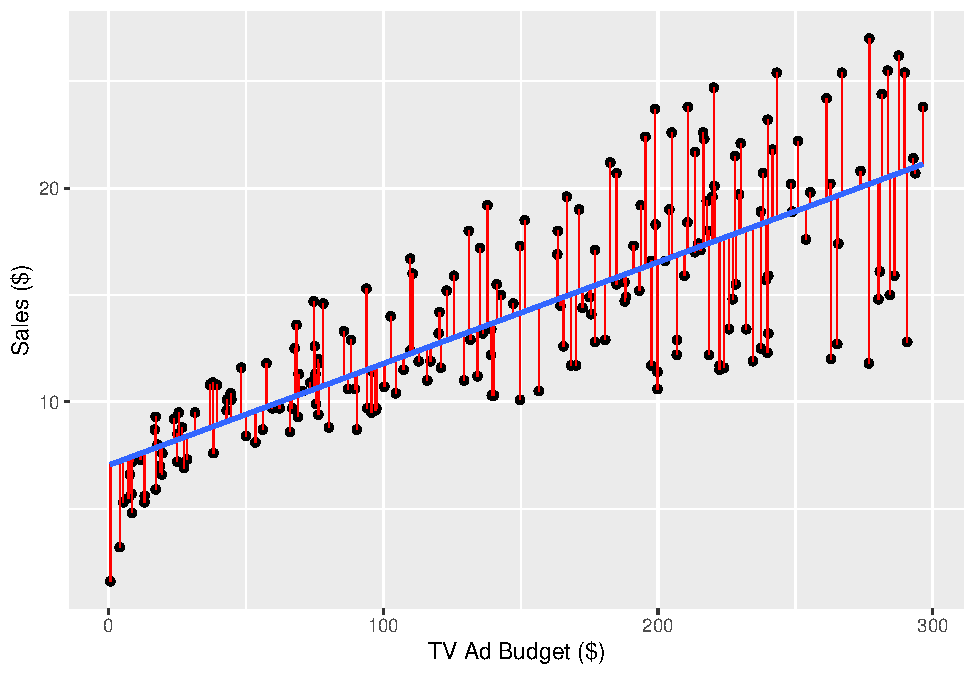
\includegraphics{Types-of-Regressions_files/figure-latex/unnamed-chunk-15-1.pdf}

As mentioned earlier, the linear regression assumption are linearity,
normality of residuals, Homogeneity of residual variance and the
independence of the residual error terms.

\hypertarget{diagnostic-plot.}{%
\subsubsection{3.1 Diagnostic Plot.}\label{diagnostic-plot.}}

The base function \emph{plot()} or the \emph{autoplot()} function from
\emph{ggfortify} package can be used to plot regression diagnostic plots
as follows;

\begin{lstlisting}[language=R]
> library(ggfortify)
> autoplot(slrTV)
\end{lstlisting}

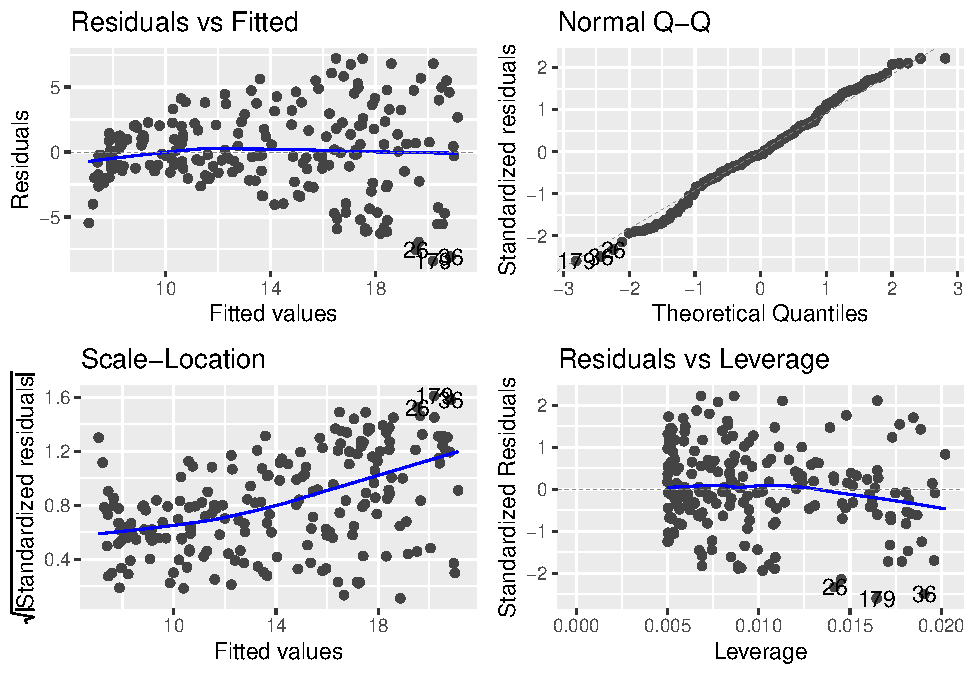
\includegraphics{Types-of-Regressions_files/figure-latex/unnamed-chunk-16-1.pdf}

\textbf{1.The Residual vs Fitted plot}- It used to check linear
relationship assumption. An approximate horizontal line without distinct
pattern is a good indication of linear relationship.

\textbf{2. The Normal Q-Q Plot}- This plot is used to check whether the
residuals are normally distributed. The residual terms should follow the
straight dashed line to satisfy the assumption.

**\emph{3. The Scale-Location Plot}- It used to check whether the
residuals have a constant variance( homoscedasticity). A horizontal line
with equally spread points is an indication of a constant variance which
is not the case in our plot. The plot indicates that the variance of the
residuals is heteroscedastic, which should be dealt with.

\textbf{4. Residuals vs Leverage Plot}- It is used to check extreme
values that may affect the regression.Outliers may affect the
interpretation of the model since they increase the RSE of the model.

For our case, the plot shows that there is linear relationship and that
the residuals are normally distributed. Let us check the high leverage
values and influential values.

\begin{lstlisting}[language=R]
> plot(slrTV, 5)
\end{lstlisting}

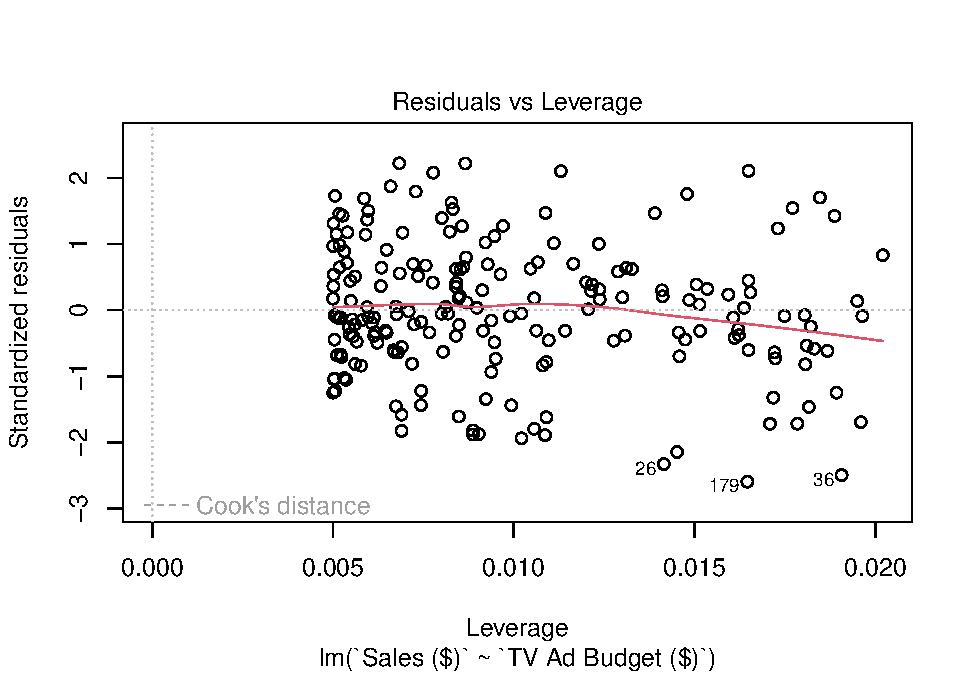
\includegraphics{Types-of-Regressions_files/figure-latex/unnamed-chunk-17-1.pdf}

A data point has a high leverage if it has an extreme predictor variable
values. A data point above the statistic

\[\frac{2(p+1)}{n}\]

(where p is the number of predictors and n is the number of
observations) indicates an observation with high leverage. In our case,
the statistic is

\[\frac{2*2}{200}=0.02\]

The plot above indicates outliers on the 26, 36 and 179 which have a
standardized error below -2, however none exceed a standard deviation of
3. All the observations are below 0.02, hence there are no observations
with high leverage.

An influential value is a value which may alter the regression if it is
included or excluded in the building of model. Note that not all ouliers
are influential values. An observation has influence if its Cook's
distance (P. Bruce and Bruce 2017) exceeds;

\[\frac{4}{n-p-1}\].

\begin{lstlisting}[language=R]
> par(mfrow = c(1, 2))
> plot(slrTV, 4)
> plot(slrTV, 5)
\end{lstlisting}

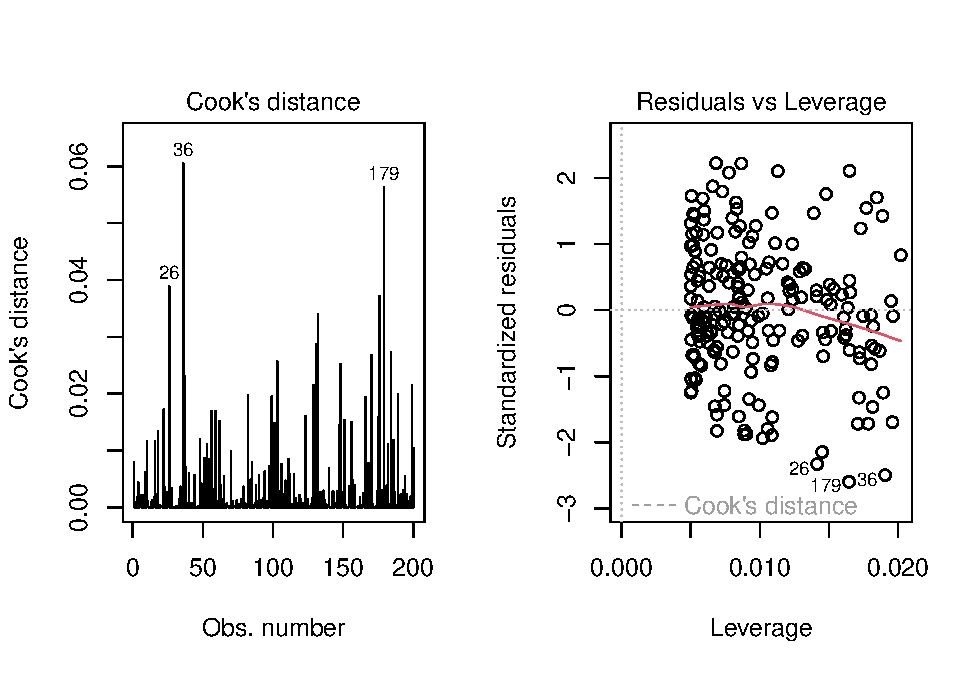
\includegraphics{Types-of-Regressions_files/figure-latex/unnamed-chunk-18-1.pdf}

In our case, we do not have influential values, the cooks distance
(represented by a red dotted line) is not drawn in the above plot
because all the observations are well within the Cooks distance.

From the plot below, there is heteroscedasticity. This can be eliminated
by transforming the data in various ways such as log transformation of
the response variable.

\begin{lstlisting}[language=R]
> plot(slrTV, 3)
\end{lstlisting}

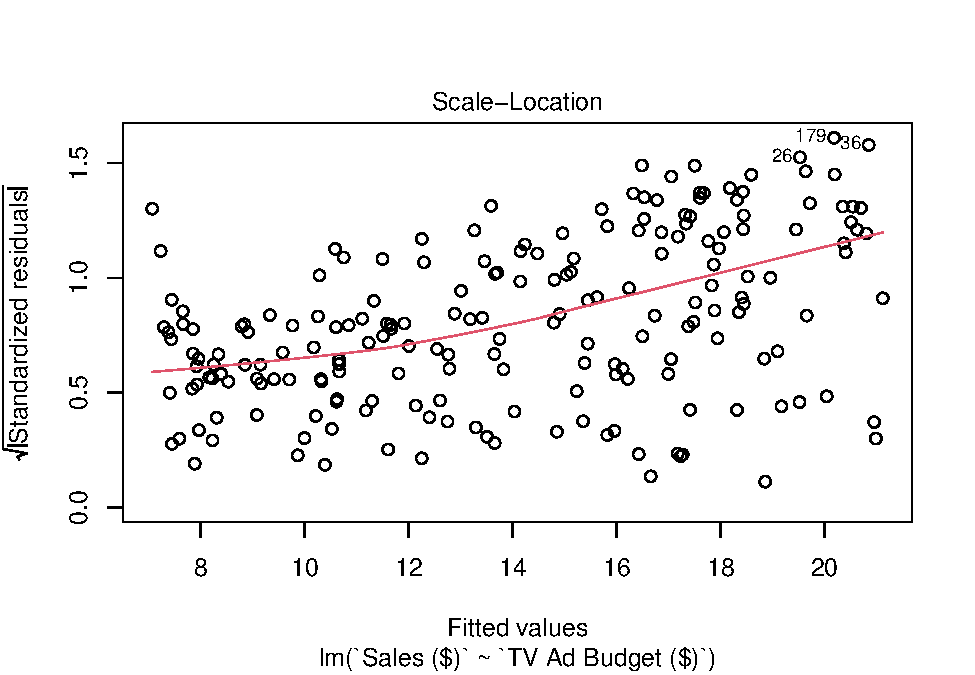
\includegraphics{Types-of-Regressions_files/figure-latex/unnamed-chunk-19-1.pdf}

\begin{lstlisting}[language=R]
> slrTVlog <- lm(log(`Sales ($)`) ~ `TV Ad Budget ($)`, data = AdvertisingBudgetandSales)
> plot(slrTVlog, 3)
\end{lstlisting}

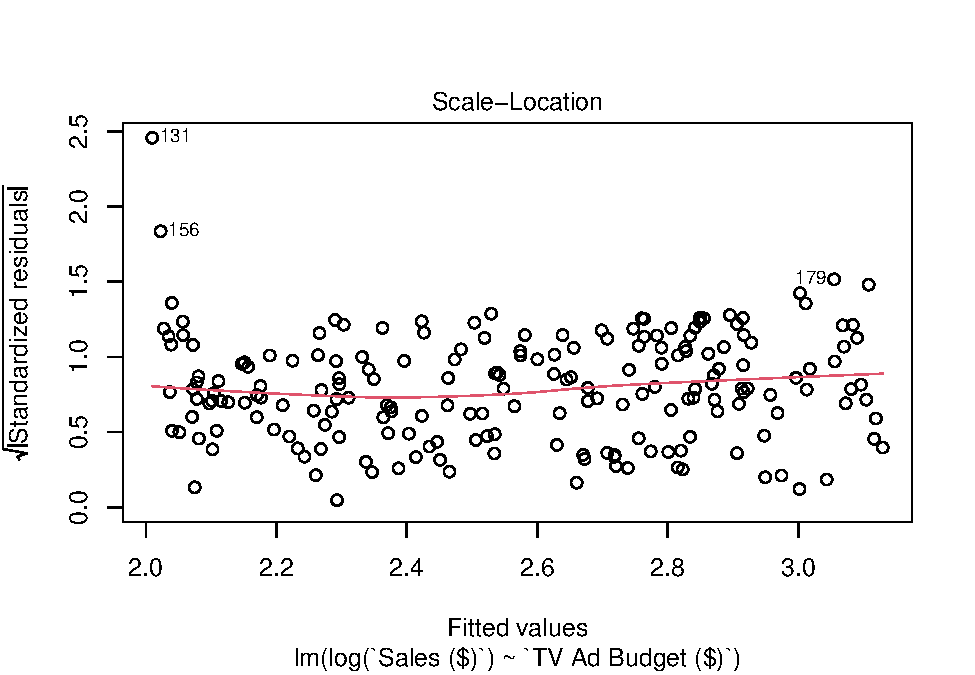
\includegraphics{Types-of-Regressions_files/figure-latex/unnamed-chunk-20-1.pdf}

From the plot above, the variance of the residual is homoscedastic.

\newpage

\hypertarget{interaction-effect-in-multiple-linear-regression}{%
\section{4.0 Interaction Effect in Multiple Linear
Regression}\label{interaction-effect-in-multiple-linear-regression}}

The multiple linear regression \(sales=2.921+0.046TV+0.188Radio\) is
also known as an \textbf{additive model}. This model only investigates
the main effects of the model, where the assumption is that the
relationship between one predictor variable and the response variable is
independent of the other predictor variables. For example, in the above
model, the effect on sales due to TV advertisement is independent of
Radio advertisement which might not be true. It can be the case that
spending money on TV advertisement may also increase the Radio
advertisement effectiveness. In business, this is known as
\textbf{synergy} while in statistics it is known as \emph{interaction
effect}. Generally, the model is written as (assuming we have two
independent variables);

\[\hat{y_i}=\hat{\beta_0}+\hat{\beta_1}x_1+\hat{\beta_2}x_2+\hat{\beta_3}x_1x_2\]

In r, we can build an interaction model as follows;

\begin{lstlisting}[language=R]
> mlrinteract <- lm(`Sales ($)` ~ `TV Ad Budget ($)` + `Radio Ad Budget ($)` + `TV Ad Budget ($)`:`Radio Ad Budget ($)`,
+     data = AdvertisingBudgetandSales)
\end{lstlisting}

Or alternatively

\begin{lstlisting}[language=R]
> mlrinteract <- lm(`Sales ($)` ~ `TV Ad Budget ($)` * `Radio Ad Budget ($)`, data = AdvertisingBudgetandSales)
> ## Both ways will build the interaction model Let us have glimpse of the model
> ## metrics
> 
> summary(mlrinteract)
\end{lstlisting}

\begin{lstlisting}
## 
## Call:
## lm(formula = `Sales ($)` ~ `TV Ad Budget ($)` * `Radio Ad Budget ($)`, 
##     data = AdvertisingBudgetandSales)
## 
## Residuals:
##     Min      1Q  Median      3Q     Max 
## -6.3366 -0.4028  0.1831  0.5948  1.5246 
## 
## Coefficients:
##                                           Estimate Std. Error t value Pr(>|t|)
## (Intercept)                              6.750e+00  2.479e-01  27.233   <2e-16
## `TV Ad Budget ($)`                       1.910e-02  1.504e-03  12.699   <2e-16
## `Radio Ad Budget ($)`                    2.886e-02  8.905e-03   3.241   0.0014
## `TV Ad Budget ($)`:`Radio Ad Budget ($)` 1.086e-03  5.242e-05  20.727   <2e-16
##                                             
## (Intercept)                              ***
## `TV Ad Budget ($)`                       ***
## `Radio Ad Budget ($)`                    ** 
## `TV Ad Budget ($)`:`Radio Ad Budget ($)` ***
## ---
## Signif. codes:  0 '***' 0.001 '**' 0.01 '*' 0.05 '.' 0.1 ' ' 1
## 
## Residual standard error: 0.9435 on 196 degrees of freedom
## Multiple R-squared:  0.9678, Adjusted R-squared:  0.9673 
## F-statistic:  1963 on 3 and 196 DF,  p-value: < 2.2e-16
\end{lstlisting}

From the output above it can be seen that all the coefficients including
the interaction coefficient are statistically significant (Note: If the
interaction effect is statistically significant, do not try to interpret
the predictor variables independently). The model is;

\[sales=6.750220 +0.019101TV+0.028860Radio+  0.001086TV*Radio\]

This interaction is known as \textbf{two way interaction} because it is
interaction between two independent variables. High order interaction is
possible also.

If the Radio advertisement budget is zero, then;

\[sales=6.750+0.019TV\]

The above implies that if Radio budget is zero, then TV advertisement
causes an average of 0.019*1000 dollars change in sales

However, if the Radio advertisement budget is one (or \$1000 for these
case), then;

\[sales=6.750+0.019TV+0.029Tv\]

Therefore;

\[sales=6.750+0.048TV\]

The above implies that a budget of 1000 dollars in Radio advertisement,
causes a 0.048*1000 dollars change in sales.

A positive interaction in this case implies that the larger the Radio
advertisement budget, the higher the effect of TV advertisement on the
sales and similary, the larger the TV advertisement budget, the higher
the effect of Radio advertisement on sales.

\hypertarget{additive-and-interaction-models-comparison}{%
\subsubsection{4.1 Additive and Interaction Models
Comparison}\label{additive-and-interaction-models-comparison}}

The \textbf{Root Mean Square Error (RMSE)} of the additive model is;

\begin{lstlisting}[language=R]
> library(qpcR)
> RMSE(mlr2)
\end{lstlisting}

\begin{lstlisting}
## [1] 1.668703
\end{lstlisting}

While the RMSE of the interaction model is;

\begin{lstlisting}[language=R]
> RMSE(mlrinteract)
\end{lstlisting}

\begin{lstlisting}
## [1] 0.9340326
\end{lstlisting}

The lower the RMSE, the better the model. RMSE is the standard deviation
of the residuals. It is a metric that tells us the average distance
between the predicted or the fitted values and the observed or measured
values. It is calculated as;

\[RMSE=\sqrt{\frac{\sum_{i=1}^n P_i-O_i}{n-1}} \]

Also the RMSE is the square root of the Mean Square Error(MSE) where MSE
is the average of the squared differences between the observed values
and the predicted values. For example;

\begin{lstlisting}[language=R]
> anova(mlrinteract)
\end{lstlisting}

\begin{lstlisting}
## Analysis of Variance Table
## 
## Response: Sales ($)
##                                           Df Sum Sq Mean Sq F value    Pr(>F)
## `TV Ad Budget ($)`                         1 3314.6  3314.6 3723.36 < 2.2e-16
## `Radio Ad Budget ($)`                      1 1545.6  1545.6 1736.22 < 2.2e-16
## `TV Ad Budget ($)`:`Radio Ad Budget ($)`   1  382.4   382.4  429.59 < 2.2e-16
## Residuals                                196  174.5     0.9                  
##                                             
## `TV Ad Budget ($)`                       ***
## `Radio Ad Budget ($)`                    ***
## `TV Ad Budget ($)`:`Radio Ad Budget ($)` ***
## Residuals                                   
## ---
## Signif. codes:  0 '***' 0.001 '**' 0.01 '*' 0.05 '.' 0.1 ' ' 1
\end{lstlisting}

\begin{lstlisting}[language=R]
> ## MSE = 0.9 implying that RMSE=sqrt(0.9)
> 
> sqrt(0.9)
\end{lstlisting}

\begin{lstlisting}
## [1] 0.9486833
\end{lstlisting}

\begin{lstlisting}[language=R]
> RMSE(mlrinteract)
\end{lstlisting}

\begin{lstlisting}
## [1] 0.9340326
\end{lstlisting}

The Residual Standard Error or the model sigma is the variant of RMSE
adjusted for the number of predictors. Therefore, since the interaction
model has lower RMSE, it is the best model.

Also, the \(adjusted\space R^2\) of the interaction model is 0.9673
which is equivalent to 96.73\%, while that of the additive model is
0.8962 or 89.62\%, implying that the interactive model is better than
the additive model, since 96.73\% of the total variation in sales is
explained by the interactive model.

\newpage

\hypertarget{regression-model-validation.}{%
\section{5.0 Regression Model
Validation.}\label{regression-model-validation.}}

The commonly used metrics for validation of a regression model are;

\begin{enumerate}
\def\labelenumi{\arabic{enumi}.}
\item
  Root Mean Square Error (RMSE)
\item
  Residual Standard Error (RSE)
\item
  R-squared (\(R^2\))
\item
  Mean Absolute Error (MAE)
\item
  Akaike Information Criterion (AIC) or AICc
\item
  Bayesian Information Criterion (BIC)
\end{enumerate}

The first three metrics have already been discussed above.

\hypertarget{akaike-information-criterion-aic}{%
\subsection{5.1 Akaike Information Criterion
(AIC)}\label{akaike-information-criterion-aic}}

AIC was developed by a Japanese statistician Hirotugu Akaike, in 1970.
AIC penalizes the inclusion of additional variables in the model. It is
used to compare various models of the same data and determine which
model is the best. The best model is the model with the lowest AIC.
Notice that adding more parameters increases the AIC, hence the model
with fewer parameters will have the lower AIC. \footnote{Cavanaugh, J.
  E., \& Neath, A. A. (2019). The Akaike information criterion:
  Background, derivation, properties, application, interpretation, and
  refinements. Wiley Interdisciplinary Reviews: Computational
  Statistics, 11(3), e1460.}

According to AIC, the best model is the model which explains the
greatest amount of variation in the dependent variable using the fewest
possible independent variables. It is calculated as;

\[AIC=2k-2\ln{L}\]

where;

-\(k\) is the number of independent variables.

-\(L\) is the log-likelihood estimate (Likelihood that your model would
have produced the observed model)

The default number of independent variables is 2, so if you have one
independent variable, then, \(k=3\) and so on.

To use the AIC, you need to build several models and then compare them.
For example, we may build several models using the advertisement data
set and see which best explains the variations in sale. In this case, I
will build separate models for each independent variable, and then
compare it with the model for the combined independent variables (TV,
Radio and Newspaper). I had already done models for TV advert then TV,
Radio and Newspaper advert, as well as TV, Radio advert, hence I'll just
proceed to the remaining two separate models for Radio and Newspaper.

\begin{lstlisting}[language=R]
> slrRadio <- lm(`Sales ($)` ~ `Radio Ad Budget ($)`, data = AdvertisingBudgetandSales)
> slrNewspaper <- lm(`Sales ($)` ~ `Newspaper Ad Budget ($)`, data = AdvertisingBudgetandSales)
\end{lstlisting}

For clarification, I have named the models as follows;

\begin{itemize}
\item
  slrTV - TV advertisement
\item
  slrRadio - Radio Advertisement
\item
  slrNewspaper - Newspaper advertisement
\item
  mlr - model for combined TV, Radio and Newspaper advert
\item
  mlr2 - combined model for TV and Radio adverts without newspaper
\item
  mlrinteract - interaction model
\end{itemize}

I'm going to use the function \emph{aictab()} from the \emph{AICcmodavg}
package as follows;

\begin{lstlisting}[language=R]
> ## listing the models in a list
> Models <- list(slrTV, slrRadio, slrNewspaper, mlr, mlr2, mlrinteract)
> ## naming the models
> Models.names = c("slrTV", "slrRadio", "slrNewspaper", "mlr", "mlr2", "mlrinteract")
> library(AICcmodavg)
> ## Then use the function
> aictab(cand.set = Models, modnames = Models.names)
\end{lstlisting}

\begin{lstlisting}
## 
## Model selection based on AICc:
## 
##              K    AICc Delta_AICc AICcWt Cum.Wt      LL
## mlrinteract  5  550.59       0.00      1      1 -270.14
## mlr2         4  780.60     230.01      0      1 -386.20
## mlr          5  782.67     232.08      0      1 -386.18
## slrTV        3 1044.21     493.63      0      1 -519.05
## slrRadio     3 1152.80     602.21      0      1 -573.34
## slrNewspaper 3 1222.79     672.21      0      1 -608.34
\end{lstlisting}

The best fit model is always listed first. The best model for this study
is the Interaction model (Recall that it is the interaction between TV
and Radio Adverts). The AICc in the output above contains the model
information -the lower the value the better the model. The lowercase
``c'' implies that it is the AIC of small samples. The Delta\_AICc (or
Delta\_AIC) is the difference between the AICc (or AIC) of the best
model and the model being compared. LL is the log likelihood used to
calculate the AIC.

\hypertarget{bayesian-information-criterion}{%
\subsection{5.2 Bayesian Information
Criterion}\label{bayesian-information-criterion}}

It is a method for scoring and selecting a model. It is almost similar
to AIC,only that while AIC penalizes the additional parameters, BIC
penalizes the complexity.More complex models have higher BICs. The lower
the value, the better the model. It is widely used in \emph{logistic
Regression} It is calculated as;

\[BIC=-2L+\ln{N}*K\]

Where; -\(k\) is the number of independent variables.

-\(L\) is the log-likelihood estimate (Likelihood that your model would
have produced the observed model) - \(N\) is the number of observations.

\textbf{Note that AIC and BIC are best used in models fit by Maximum
Likelihood Estimation framework}

\hypertarget{mean-absolute-error-mae}{%
\subsection{5.3 Mean Absolute Error
(MAE)}\label{mean-absolute-error-mae}}

MAE is a loss function used for regression. The loss is the mean over
the absolute differences of the observed values and the predicted
values. The lower the value the better the model. It is calculated as;

\[MAE=\frac{1}{N}\sum_{i=1}^N|y-\hat{y_i}|\]

\newpage

\hypertarget{logistic-regression}{%
\section{6.0 Logistic Regression}\label{logistic-regression}}

\textbf{Logistic Regression} is used to predict the category or class of
individuals using one or multiple predictor variables. Logistic
regression estimates the probability of an event occurring, therefore,
since the outcome is probability, the dependent variable is bounded
between 0 and 1. It is used to predict the outcome of a binary (such as
yes or no) based on past values of the data. Logistic regression belongs
to the family of \textbf{Generalized Linear Models (GLM)} which was
built to extend the Linear Regression Model. Logistic Regression is also
known as \emph{binary logistic regression} ,\emph{binomial logistic
regression} or \emph{logit regression}. The model was initially
introduced by Joseph Berkson in 1944. The \emph{response variable} which
I will refer as \(Y\) in this paper, is parametarized by
\(0\space or\space 1\). Traditionally, \(1\) is indicates a
\emph{success} while \(0\) indicates a \emph{failure} or \emph{lack of
success}. \(1\) can also be thought of having a certain characteristic,
condition, requirement or property while \(0\) can be thought of having
certain characteristics or properties. This type of regression is widely
used in epidemiological data analysis. For example, we might have a
research question such as; \emph{what is the relationship between one or
more exposure variable(s) say E to a disease or illness outcome D}. Let
us further take an example of smoking habits and Coronary Heart
Disease(CHD), where the question is to which extent is CHD related with
smoking. Here, \(1\) will represent smoker and \(0\) non smoker for the
case of the independent variable smoking. Also, \(1\) will represent
\emph{diseased or having CHD} and \(0\) will represent \emph{not
diseased or not having CHD} , for the case of the response variable.

Other independent variables such as age, race and sex are known as
\textbf{control variables} (\(C_s\)) . These control variables together
with the binary variables \(E_S\) form a collection of independent
variables which are used to predict the outcome of the response
variable. More generally, as usual, the independent variables are
represented with \(X\) regardless of whether they are \(C_s\) or \(E_s\)
-\emph{Note that the subscript s is used to represent prural or many
variables}. Also, in logistic regression the dependent variable is
always a binary outcome.

It is important to note that logistic regression is based on the
logistic function below;

\[f(z)=\frac{1}{1+e^{-z}}\space\space for\space\space -\infty<z<\infty \]

The graph of this function is shown below;

\begin{lstlisting}[language=R]
> eq = function(z) {
+     1/(1 + exp(-z))
+ }
> library(ggplot2)
> base <- ggplot() + xlim(-5, 5) + ylim(-1, 1)
> base + geom_function(fun = eq, col = "red") + geom_hline(yintercept = c(0, 1), linetype = "dotted") +
+     geom_vline(xintercept = 0, linetype = "dotted")
\end{lstlisting}

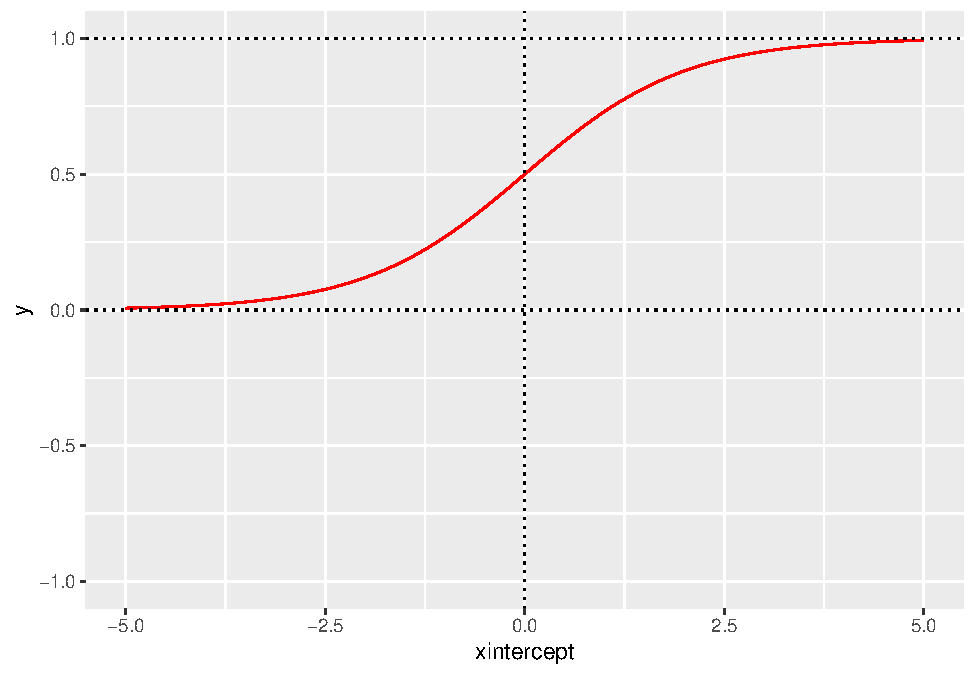
\includegraphics{Types-of-Regressions_files/figure-latex/unnamed-chunk-28-1.pdf}

Notice that for \(z=-\infty\), then \(f(z)=0\) and for \(z=\infty\),then
\(f(z)=1\). Thus the value of \(f(z)\) ranges from zero to one
regardless of the value of \(z\), which is the primary reason as to why
logistic regression is popular. As mentioned earlier, the response
variable to be predicted is a probability, and as you know probability
ranges from zero to one, hence this model is suitable.

The elongated \textbf{S} shape of the function appeals the
epidemiologists if \(z\) represents an index that combines the
contribution of several risk factors and \(f(z)\) represents the risk
for a given value of \(z\). As in most diseases and risk factors, the
logistic function shows that at low level exposure, the individual's
risk is minimal until it reaches a certain threshold after which the
risk increases rapidly, to a certain threshold also where the risk
remains extremely high.

\newpage

\hypertarget{the-logistic-model}{%
\subsection{6.1 The Logistic Model}\label{the-logistic-model}}

To obtain the logistic model, we write \(z\) as a linear sum of
\(x\space\space and \space\space \beta_i\) as follows;

\[z=\beta_0+\beta_1x_1+\beta_2x_2+\dots\beta_nx_n\]

Then, substituting for \(z\) in the logistic function above, we get;

\[f(z)=\frac{1}{(1+e^{-(\beta_0+\sum_{i=1}^n\beta_i x_i)}}\]

Assuming that \(D\) is the disease whose probability is being modeled,
then we denote \(f(z)\) as follows;

\[\mathbb{P}(D|x_1,x_2\dots x_i)=\frac{1}{(1+e^{-(\beta_0+\sum_{i=1}^n\beta_i x_i)}}\]

By multiplication, it can be shown that;

\[\frac{\mathbb{P}(D)}{1-\mathbb{P}(D)}=e^{(\beta_0+\beta_1x1+\dots+\beta_nx_n)}\]

Taking log on both sides we get;
\[\log(\frac{\mathbb{P}(D)}{1-\mathbb{P}(D)})=\beta_0+\beta_1x_1+\dots+\beta_nx_n\]

The quantity \(\log\{\frac{\mathbb{P}(D)}{1-\mathbb{P}(D)}\}\) is known
as \textbf{log-odd} or the \textbf{logit}. The \textbf{odd} refer to the
likelihood of an event occurring. It can also be seen as the ratio of
``success'' to ``non-success''.

\hypertarget{simple-logistic-model}{%
\subsubsection{6.1.1 Simple Logistic
Model}\label{simple-logistic-model}}

The simple logistic model is used to estimate the probability of class
membership based on one predictor or independent variable. The model is
written as;

\[\mathbb{P}(D|x_1)=\frac{1}{(1+e^{-(\beta_o+\beta_1x_1)})}\]

To understand this type of regression, let us use an example where let
the disease of interest \(D\) be \(CHD\) or Coronary Heart Disease. We
wish to find out whether a certain gender increases the risk of
contracting CHD. I am going to use a data set publicly available on
\emph{Kaggle}. The data set is from a study of cardiovascular study on
residents of the town of Framingham, Massachusetts, which recorded
whether the persons in the study contracted CHD.

\begin{lstlisting}[language=R]
> ## Importing the data
> setwd("D:/Documents/R-Studio Programms/Regression/Logistic Regression")
> library(readxl)
> CHD <- read_excel("CHD.xlsx")
> 
> head(CHD)
\end{lstlisting}

\begin{lstlisting}
## # A tibble: 6 x 10
##   Gender   age currentSmoker cigsPerDay   Hyp  Chol   BMI heartRate glucose
##    <dbl> <dbl>         <dbl>      <dbl> <dbl> <dbl> <dbl>     <dbl>   <dbl>
## 1      1    39             0          0     0   195  27.0        80      77
## 2      0    46             0          0     0   250  28.7        95      76
## 3      1    48             1         20     0   245  25.3        75      70
## 4      0    61             1         30     1   225  28.6        65     103
## 5      0    46             1         23     0   285  23.1        85      85
## 6      0    43             0          0     1   228  30.3        77      99
## # ... with 1 more variable: CHD <dbl>
\end{lstlisting}

\begin{lstlisting}[language=R]
> ## Data Preparation
> CHD$Gender <- factor(CHD$Gender, levels = c(0, 1), labels = c("Female", "Male"))
> CHD$currentSmoker <- factor(CHD$currentSmoker, levels = c(0, 1), labels = c("No",
+     "Yes"))
> CHD$Hyp <- factor(CHD$Hyp, levels = c(0, 1), labels = c("No", "Yes"))
> 
> CHD$CHD <- factor(CHD$CHD, levels = c(0, 1), labels = c("No", "Yes"))
> model1 <- glm(CHD ~ Gender, family = binomial, data = CHD)
> summary(model1)
\end{lstlisting}

\begin{lstlisting}
## 
## Call:
## glm(formula = CHD ~ Gender, family = binomial, data = CHD)
## 
## Deviance Residuals: 
##     Min       1Q   Median       3Q      Max  
## -0.6504  -0.6504  -0.5142  -0.5142   2.0440  
## 
## Coefficients:
##             Estimate Std. Error z value Pr(>|z|)    
## (Intercept) -1.95676    0.06600 -29.647  < 2e-16 ***
## GenderMale   0.51075    0.09058   5.639 1.71e-08 ***
## ---
## Signif. codes:  0 '***' 0.001 '**' 0.01 '*' 0.05 '.' 0.1 ' ' 1
## 
## (Dispersion parameter for binomial family taken to be 1)
## 
##     Null deviance: 3257.3  on 3799  degrees of freedom
## Residual deviance: 3225.3  on 3798  degrees of freedom
## AIC: 3229.3
## 
## Number of Fisher Scoring iterations: 4
\end{lstlisting}

In logistic model, a negative intercept (\(\beta_0\)) implies that the
probability of having the disease or the outcome is below 0.5. A
positive intercept implies that the probability of having the disease or
the outcome is greater than 0.5, while an intercept equal to zero
implies that the probability is approximately equal to 0.5.

From the output above, our model can be written as;

\[\mathbb{P}(CHD|gender)=\frac{1}{(1+e^{-(1.957+0.511gender)})}\]

The probability of CHD infection given that you are a male is;

\[\mathbb{P}(CHD|gender)=\frac{1}{(1+e^{-(-1.957+0.511*1)})}=0.191\]

And the probability of CHD infection given that you are a female is;

\[\mathbb{P}(CHD|gender)=\frac{1}{(1+e^{-(1.951+0.492*0)})}=0.124\]

From the above calculations we can conclude that the risk of having CHD
is higher for males than for females. Then if we divide the predicted
risk of males by the predicted risk of females as shown below, we obtain
the \textbf{risk ratio estimate} \(\hat{RR}\).

\[\frac{\mathbb{P}(CHD|male)}{\mathbb{P}(CHD|female)}=\frac{0.191}{0.124}=1.540\]

Thus using the the fitted model above we find that risk of males
contracting CHD is one and half times the risk of females contracting
CHD. More information can be obtained by the summary function in r.

\begin{lstlisting}[language=R]
> summary(model1)
\end{lstlisting}

\begin{lstlisting}
## 
## Call:
## glm(formula = CHD ~ Gender, family = binomial, data = CHD)
## 
## Deviance Residuals: 
##     Min       1Q   Median       3Q      Max  
## -0.6504  -0.6504  -0.5142  -0.5142   2.0440  
## 
## Coefficients:
##             Estimate Std. Error z value Pr(>|z|)    
## (Intercept) -1.95676    0.06600 -29.647  < 2e-16 ***
## GenderMale   0.51075    0.09058   5.639 1.71e-08 ***
## ---
## Signif. codes:  0 '***' 0.001 '**' 0.01 '*' 0.05 '.' 0.1 ' ' 1
## 
## (Dispersion parameter for binomial family taken to be 1)
## 
##     Null deviance: 3257.3  on 3799  degrees of freedom
## Residual deviance: 3225.3  on 3798  degrees of freedom
## AIC: 3229.3
## 
## Number of Fisher Scoring iterations: 4
\end{lstlisting}

The \textbf{null deviance} above is a concept in generalized linear
models that measures the fitted generalized model against a perfect
model known as the \textbf{saturated model}. It is a generalization of
the total sums of squares in a linear model. The null deviance shows how
well the model predicts the response variable with the intercept only.
The smaller the Null Deviance, the better the model.

The \textbf{residual deviance} shows how well a model can predict the
response variable with more than -say \(p\)- predictors. To determine
the usefulness of the model we can calculate a \(\chi^2\) statistic with
\(p\) (number of predictor variables) degrees of freedom as follows;
Note that, the lower the value of residual deviance, the better the
model (Obviously)

\[\chi^2_{(p)}=Null\space deviance\space -\space Residual\space deviance\]

After which we find the p-value associated with the statistic, if it is
less than \(\alpha=0.05\) (for our case), then the model is useful or
significant. We only have one predictor variable, thus the degrees of
freedom = 1.

\[\chi^2_{(1)}= 3257.3-3225.3=32\]

\begin{lstlisting}[language=R]
> pchisq(q = 32, df = 1, lower.tail = F)
\end{lstlisting}

\begin{lstlisting}
## [1] 1.541726e-08
\end{lstlisting}

Thus since the p-value is less than \(\alpha\), our model is useful.

\hypertarget{multiple-logistic-regression}{%
\subsubsection{6.1.2 Multiple Logistic
Regression}\label{multiple-logistic-regression}}

The procedure for multiple logistic regression is the same as for the
simple logistic regression. A multiple logistic regression is logistic
regression where more than one predictor variables are used to predict
the response variable. For example, we may wish to know the effect of
age, hypertension, gender, heart rate, smoking habit, BMI level,
cholesterol levels and glucose levels on contracting CHD. In r, we build
a multiple logistic model as follows;

\begin{lstlisting}[language=R]
> model2 <- glm(CHD ~ Gender + age + heartRate + cigsPerDay + Hyp + glucose + Chol +
+     BMI, family = binomial, data = CHD)
> summary(model2)
\end{lstlisting}

\begin{lstlisting}
## 
## Call:
## glm(formula = CHD ~ Gender + age + heartRate + cigsPerDay + Hyp + 
##     glucose + Chol + BMI, family = binomial, data = CHD)
## 
## Deviance Residuals: 
##     Min       1Q   Median       3Q      Max  
## -1.9710  -0.6124  -0.4272  -0.2864   2.7772  
## 
## Coefficients:
##              Estimate Std. Error z value Pr(>|z|)    
## (Intercept) -7.836466   0.591433 -13.250  < 2e-16 ***
## GenderMale   0.494717   0.104323   4.742 2.11e-06 ***
## age          0.071724   0.006166  11.631  < 2e-16 ***
## heartRate   -0.001034   0.004091  -0.253   0.8004    
## cigsPerDay   0.020985   0.004120   5.094 3.51e-07 ***
## HypYes       0.626856   0.103172   6.076 1.23e-09 ***
## glucose      0.008224   0.001651   4.981 6.33e-07 ***
## Chol         0.002920   0.001060   2.753   0.0059 ** 
## BMI          0.015999   0.011882   1.346   0.1782    
## ---
## Signif. codes:  0 '***' 0.001 '**' 0.01 '*' 0.05 '.' 0.1 ' ' 1
## 
## (Dispersion parameter for binomial family taken to be 1)
## 
##     Null deviance: 3257.3  on 3799  degrees of freedom
## Residual deviance: 2901.5  on 3791  degrees of freedom
## AIC: 2919.5
## 
## Number of Fisher Scoring iterations: 5
\end{lstlisting}

From the output above, we can see that most predictor variables are
significant at \(1\%\) level of significance. However, the predictor
variables named heartRate and BMI levels are not significant and should
be eliminated to increase the accuracy of the model. This elimination
can be automatically using statistical techniques, including
\textbf{step-wise regression} and \textbf{penalized regression}.

\begin{lstlisting}[language=R]
> model3 <- glm(CHD ~ Gender + age + cigsPerDay + Hyp + glucose + Chol, family = binomial,
+     data = CHD)
> summary(model3)
\end{lstlisting}

\begin{lstlisting}
## 
## Call:
## glm(formula = CHD ~ Gender + age + cigsPerDay + Hyp + glucose + 
##     Chol, family = binomial, data = CHD)
## 
## Deviance Residuals: 
##     Min       1Q   Median       3Q      Max  
## -2.0158  -0.6121  -0.4270  -0.2878   2.7786  
## 
## Coefficients:
##              Estimate Std. Error z value Pr(>|z|)    
## (Intercept) -7.517672   0.430433 -17.465  < 2e-16 ***
## GenderMale   0.504079   0.103277   4.881 1.06e-06 ***
## age          0.071662   0.006156  11.642  < 2e-16 ***
## cigsPerDay   0.020410   0.004074   5.010 5.45e-07 ***
## HypYes       0.659169   0.098367   6.701 2.07e-11 ***
## glucose      0.008344   0.001646   5.069 4.00e-07 ***
## Chol         0.002933   0.001057   2.776  0.00551 ** 
## ---
## Signif. codes:  0 '***' 0.001 '**' 0.01 '*' 0.05 '.' 0.1 ' ' 1
## 
## (Dispersion parameter for binomial family taken to be 1)
## 
##     Null deviance: 3257.3  on 3799  degrees of freedom
## Residual deviance: 2903.3  on 3793  degrees of freedom
## AIC: 2917.3
## 
## Number of Fisher Scoring iterations: 5
\end{lstlisting}

Thus our model can be written as;

\[\mathbb{P}(CHD|gender,\dots)=\frac{1}{(1+e^{-(-7.518+0.504Gender+0.071Age+0.020CigsPerDay+0.660Hyp+0.008glucose+0.003Cholestrol)})}\]

From the output above, we see that all the \(\beta\) coefficients of
predictor variables are positive which implies that if any of the
predictor variables is increased, the probability of having CHD
increases (This applies for the control predictor variables) We can also
calculate the odds ratio by taking the exponential of the predictor
variables. For example, the \(\beta\) coefficient for glucose is
\(0.008\) which implies that a one unit increase in glucose will
increase the odds of having CHD by \(e^{0.008}=1.008\) times. Number of
iterations is just a measure of how long it took to fit your model and
you can safely ignore it.

Note that, we only estimate the Risk Ratio using the logistic regression
if a follow up study was conducted. However, in the case of
Cross-sectional and case control study, we cannot use the logistic
regression to estimate the individual risks but only the odds ratio. In
follow-up study, it is commonly preferred to estimate the Risk Ratio
rather than the Odds Ratio.

\newpage

\hypertarget{multinomial-logistic-regression}{%
\section{7.0 Multinomial Logistic
Regression}\label{multinomial-logistic-regression}}

A \textbf{Multinomial Logistic Regression} is an extension of the
logistic regression which is used when the outcome involves more than
two classes. It allows for more than two categories of the dependent or
the independent variable. Multinomial logistic regression is often
considered an attractive analysis because it does not assume normality,
linearity or homoscedasticity. However, it does have an assumption of
independence of choices in the dependent variable which states that the
choice of or membership in one category is not related to the choice or
membership of another category(IIA). This assumption can be tested using
the \textbf{Hausman-McFadden test}, in r, we use the function
\textbf{hmftest}, from \textbf{mlogit} package. Given that the
categorical response variable \(Y\) has more than two possible levels,
namely \({1,\dots,J}\) and further given that we have
\(X_1,X_2,\dots,X_P\), then the multiple logistic regression models the
probability of each level \(j\) of \(Y\), by;

\[p_J(\mathbf{x}):=\mathbb{P}(Y=j|X_1=x_p,\dots,X_p=x_p)=\frac{1}{(1+\sum_{\ell=1}^{J-1}e^{(\beta_{0\ell}+\beta_{1\ell}X_1+\dots+\beta_{p\ell}X_p)}}\]

The multinomial regression has an interesting interpretation of logistic
regression. For example taking the quotients;

\[\frac{p_j(\mathbf{x})}{p_J(\mathbf{x})}= e^{\beta_{0j}+\beta_{1j}X_1+\dots+\beta_{pj}X_p}\space for\space j=1,\dots,J-1\]

Then taking logarithms on both sides we get;

\[\log{(\frac{p_j(\mathbf{x})}{p_J(\mathbf{x})})}=\beta_{0j}+\beta_{1j}X_1+\dots+\beta_{pj}X_p\]

Thus, if the probabilities on LHS added to one, we would have gotten a
log-odds and hence the logistic regression for \(Y\), which is not the
case. Therefore, due to this effect, we have the \emph{ratios} or the
\emph{log-ratios} of the non-complimentary probabilities. Further,
\(e^{\beta_{0j}}\) is the ratio between \(p_j(\mathbf{0})\) and
\(p_J(\mathbf{0})\), representing the probabilities of \(Y=j\) when
\(X_1=X_2=\dots=X_p=0\).\footnote{monimal \emph{in plural monomials} is
  an algebraic expression consisting of one term.} Note the following;

\begin{enumerate}
\def\labelenumi{\arabic{enumi}.}
\item
  If \(e^{\beta_{0j}}>1\) and \(\beta_{0j}>0\), then the \(Y=j\) is more
  likely than \(Y=J\)
\item
  However, if \(e^{\beta_{0j}}<1\) and \(\beta_{0j}<0\), then \(Y=j\) is
  less likely than \(Y=J\)
\item
  \(e^{\beta_{\ell j}}\) is the \textbf{multiplicative} increment of the
  ratio between \(p_j(\mathbf{x})\) and \(p_J(\mathbf{x})\) for an
  increment in one unit of \(X_\ell=x_\ell\), provided that the
  remaining variables; \(X_1,\dots,X_{\ell-1},X_{\ell+1},\dots,X_p\) do
  not change.
\item
  If \(e^{\beta_{\ell j}}>1\) and equivalently, \(\beta_{\ell j}>0\),
  then \(Y=j\) becomes more likely than \(Y=J\) for each increment in
  \(X_j\).
\item
  if \(e^{\beta_{\ell j}}<1\) and \(\beta_{\ell j}<00\), then \(Y=j\)
  becomes less likely than \(Y=J\) for each increment in \(X_j\).
\end{enumerate}

\hypertarget{examples-of-multinomial-logistic-regression}{%
\subsection{7.1 Examples of Multinomial Logistic
Regression}\label{examples-of-multinomial-logistic-regression}}

\begin{enumerate}
\def\labelenumi{\arabic{enumi}.}
\item
  People's occupation choices might be influenced by their parents'
  occupation and their own educational level. We can model or study the
  relationship between one's occupation, educational level and the
  father's or mother's occupation. The outcome or the response variable
  will be the occupation choices which consists of occupational
  categories.
\item
  A biologist may be interested in the food choices an alligator makes.
  Adult alligators might have different choices from younger ones. Here,
  the response variable will be the food choices while the predictor
  variables can be the size of alligators (which is continuous) and
  other environmental factors.
\item
  High school students makes a program choice among general program,
  vocational program and academic program. Their choice might be modeled
  based on their writing score and social economic status.
\end{enumerate}

In r, there are various packages with inbuilt functions for building a
multinomial logistic regression, but am going to use the \textbf{nnet
package}. Let's us model the student program choice based on their
writing score and social economic status. I'm first going to download
the data set known as \textbf{hsbdemo} from
\href{https://stats.idre.ucla.edu}{stats idre website}

\begin{lstlisting}[language=R]
> require(foreign)
> require(nnet)
> require(ggplot2)
> require(reshape2)
> 
> ## downloading the data
> Student <- read.dta("https://stats.idre.ucla.edu/stat/data/hsbdemo.dta")
> 
> ## A glimpse of the first few rows of the data
> head(Student)
\end{lstlisting}

\begin{lstlisting}
##    id female    ses schtyp     prog read write math science socst       honors
## 1  45 female    low public vocation   34    35   41      29    26 not enrolled
## 2 108   male middle public  general   34    33   41      36    36 not enrolled
## 3  15   male   high public vocation   39    39   44      26    42 not enrolled
## 4  67   male    low public vocation   37    37   42      33    32 not enrolled
## 5 153   male middle public vocation   39    31   40      39    51 not enrolled
## 6  51 female   high public  general   42    36   42      31    39 not enrolled
##   awards cid
## 1      0   1
## 2      0   1
## 3      0   1
## 4      0   1
## 5      0   1
## 6      0   1
\end{lstlisting}

The response variable will be the program -named prog in the data set-
while the predictor variables will be social economic status -named ses-
which is a three-level categorical variable, writing score -named
write-a continuous variable.

First, we need to choose our level of outcome that we wish to use as our
baseline and then specify this with \textbf{relevel} function.

\begin{lstlisting}[language=R]
> Student$prog2 <- relevel(Student$prog, ref = "academic")
\end{lstlisting}

After specifying our baseline level of outcome, We can now use the
function \textbf{multinom} from the \textbf{nnet} package to build the
model.

\begin{lstlisting}[language=R]
> mlt <- multinom(prog2 ~ ses + write, data = Student)
\end{lstlisting}

\begin{lstlisting}
## # weights:  15 (8 variable)
## initial  value 219.722458 
## iter  10 value 179.982880
## final  value 179.981726 
## converged
\end{lstlisting}

\begin{lstlisting}[language=R]
> summary(mlt)
\end{lstlisting}

\begin{lstlisting}
## Call:
## multinom(formula = prog2 ~ ses + write, data = Student)
## 
## Coefficients:
##          (Intercept)  sesmiddle    seshigh      write
## general     2.852198 -0.5332810 -1.1628226 -0.0579287
## vocation    5.218260  0.2913859 -0.9826649 -0.1136037
## 
## Std. Errors:
##          (Intercept) sesmiddle   seshigh      write
## general     1.166441 0.4437323 0.5142196 0.02141097
## vocation    1.163552 0.4763739 0.5955665 0.02221996
## 
## Residual Deviance: 359.9635 
## AIC: 375.9635
\end{lstlisting}

The \emph{multinom} function, does not automatically calculate the
p-values, hence we will do it manually as follows;

\begin{lstlisting}[language=R]
> z <- summary(mlt)$coefficients/summary(mlt)$standard.errors
> z
\end{lstlisting}

\begin{lstlisting}
##          (Intercept)  sesmiddle   seshigh     write
## general     2.445214 -1.2018081 -2.261334 -2.705562
## vocation    4.484769  0.6116747 -1.649967 -5.112689
\end{lstlisting}

We can then proceed to calculate the 2-tailed z-test

\begin{lstlisting}[language=R]
> p <- (1 - pnorm(abs(z), 0, 1)) * 2
> p
\end{lstlisting}

\begin{lstlisting}
##           (Intercept) sesmiddle    seshigh        write
## general  0.0144766100 0.2294379 0.02373856 6.818902e-03
## vocation 0.0000072993 0.5407530 0.09894976 3.176045e-07
\end{lstlisting}

\hypertarget{interpretation-of-the-output}{%
\subsubsection{7.1.1 Interpretation of the
output}\label{interpretation-of-the-output}}

The model summary output has a block of coefficients and a block of
standard errors. Focusing on the block of coefficients, each row
contains a model equation. The first row compares the general program to
our baseline academic program while the second row compares the vocation
programs to academic program. Let the coefficients from the first row be
\(\hat{\beta_1}\) and further let coefficients from the second row be
\(\hat{\beta_2}\), then we can write our model as;

\[\ln(\frac{\mathbb{P}(Program=general)}{\mathbb{P}(Program=academic)})=\hat{\beta_{10}}+\hat{\beta_{11}}(ses=middle)+\hat{\beta_{12}}(ses=high)+\hat{\beta_{13}}write\]

\[\ln(\frac{\mathbb{P}(Program=general)}{\mathbb{P}(Program=academic)})=2.852-0.533(ses=middle)-1.163(ses=high)-0.058write\]

This can be interpreted as:

\begin{itemize}
\item
  A one unit increase in write leads to 0.058 decrease in the log odds
  of being in general program versus academic program.
\item
  The log odds of being in general program vs academic program decreases
  by an average of 1.163 if the student has a high social economic
  status.Or, a high class social economic status student is less likely
  to be in the general program than to be in the academic program
\item
  The log odds of being in general program vs academic program decreases
  by 0.533 if the student has a middle social economic status. Or, a
  middle class social economic status student is less likely to be in
  the general program than to be in the academic program (although not
  significant).
\item
  Since our \(\hat{\beta_{10}}>0\), then, a student is more likely to be
  in the general program than to be in the academic program, in the
  absence of other predictor variables.
\end{itemize}

Now let the coefficients from the second row be \(\hat{\beta_2}\), then
we can write the model as;

\[\ln(\frac{\mathbb{P}(Program=vocation)}{\mathbb{P}(Program=academic)})=\hat{\beta_{20}}+\hat{\beta_{21}}(ses=middle)+\hat{\beta_{22}}(ses=high)+\hat{\beta_{23}}write\]

\[\ln(\frac{\mathbb{P}(Program=vocation)}{\mathbb{P}(Program=academic)})=5.219+0/291(ses=middle)-0.983(ses=high)-0.114write\]

This can be interpreted as;

\begin{itemize}
\item
  A one unit increase in write leads to 0.114 decrease in the log odds
  of being in vocation program versus academic program.
\item
  The log odds of being in vocation program vs academic program
  decreases by 0.983 if the student has a high class social economic
  status. Or, a high class social economic status student is less likely
  to be in the vocation program than to be in the academic program.
\item
  The log odds of being in vocation program vs academic program
  increases by 0.291 if the student has a middle social economic status.
  Or, a middle class social economic status student is more likely to be
  in the vocation program than to be in the academic program (although
  not statistically significant looking at its p-value).
\item
  Since our \(\hat{\beta_{20}}>0\), then, a student is more likely to be
  in the vocation program than to be in the academic program, in the
  absence of other predictor variables.
\end{itemize}

Then the ratio of the probability of choosing one variable outcome over
another is called the relative risk. We obtain it by exponentiation of
the Right Hand Side of the model.

\begin{lstlisting}[language=R]
> exp(coef(mlt))
\end{lstlisting}

\begin{lstlisting}
##          (Intercept) sesmiddle   seshigh     write
## general     17.32582 0.5866769 0.3126026 0.9437172
## vocation   184.61262 1.3382809 0.3743123 0.8926116
\end{lstlisting}

\hypertarget{assumptions-of-the-multinomial-logistic-regression}{%
\subsubsection{7.1.2 Assumptions of the Multinomial Logistic
Regression}\label{assumptions-of-the-multinomial-logistic-regression}}

\begin{enumerate}
\def\labelenumi{\arabic{enumi}.}
\item
  The \textbf{Independence of the Irrelevant Alternatives (IIA)}- The
  IIA assumption means that deleting or removing alternative outcome
  (response) categories does not affect the odds among the remaining
  outcomes.
\item
  Sample size- The multinomial logistic regression uses the Maximum
  Likelihood Estimation method which requires a large sample size. It
  also uses multiple equations which implies that it requires a larger
  sample size than what a binary logistic regression would require.
\item
  Complete or quasi-complete separation- Complete separation means that
  the outcome variable separate a predictor variable completely, leading
  perfect prediction by the predictor variable.
\end{enumerate}

You can also use the predicted or estimated probabilities to help you
understand your model better as follows;

\begin{lstlisting}[language=R]
> head(pp <- fitted(mlt))
\end{lstlisting}

\begin{lstlisting}
##    academic   general  vocation
## 1 0.1482764 0.3382454 0.5134781
## 2 0.1202017 0.1806283 0.6991700
## 3 0.4186747 0.2368082 0.3445171
## 4 0.1726885 0.3508384 0.4764731
## 5 0.1001231 0.1689374 0.7309395
## 6 0.3533566 0.2377976 0.4088458
\end{lstlisting}

\newpage

\hypertarget{ordinal-logistic-regression}{%
\section{8.0 Ordinal Logistic
Regression}\label{ordinal-logistic-regression}}

Ordinal logistic regression is a statistical analysis method used to
model the relationship between an \textbf{ordinal response variable} and
one or more predictor variable(s). Ordinal data is a type of qualitative
type of data with a natural ordered scale e.g the level of income can be
low, middle or high. The flowchart below shows the types of data.

In r, we can use the \textbf{polr} command from \textbf{Mass} package to
build an Ordinal logistic regression. The command name comes from
proportional odds logistic regression.

\newpage

\hypertarget{polynomial-regression}{%
\section{9.0 Polynomial Regression}\label{polynomial-regression}}

In some cases, the relationship between the response variable \(y\) and
the independent or predictor variable or variables might not be linear.
In a such a case, we cannot apply the linear regression analysis as the
assumption of linearity is violated. Thus, the \textbf{Polynomial
Regression} is a type of regression whereby the relationship between the
response variable and the predictor variables is modeled as the
\(n^{th}\) degree polynomial. The polynomial regression fits a
non-linear relationship between the values of the independent variable
\(X\) and the conditional mean of \(y\) which is denoted as
\(\mathbf{E}(y|x)\). Although the polynomial regression fits a nonlinear
model to the data, as a statistical estimation problem it is linear in
the sense that the conditional mean of \(y\) i.e \(\mathbf{E}(y|x)\) is
linear to the unknown to the parameters estimated from the data, hence
it is referred to as a special case of multilple linear regression.

With polynomial regression, data is approximated using a polynomial
equation of degree \(n\) written as;

\[\mathbf{f(x)}=\alpha_0+\alpha_1x+\alpha_2x_1+\dots+\alpha_nx^n\]

where \(\alpha\) is the set of coefficients.

Now the polynomial regression equation can be written as;

\[y=\beta_0+\beta_1x_i+\beta_2x_i^2+\dots+\beta_nx_i^m+\epsilon_i \\for\space i=1,2,3,\dots,n\]

The above model can be expressed matrix form in terms of a design matrix
\(\mathbb{x}\), response vector \(\vec{y}\), the parameter vector
\(\vec{\beta}\) and the random vector \(\vec{\epsilon }\), as follows;

\[\begin{bmatrix}y_1\\y_2\\y_3\\\vdots\\y_n \end{bmatrix}=\begin{bmatrix}1&x_1&x_2^2&\dots&x_n^m\\1&x_2&x_2^2&\dots&x_2^m\\1&x_3&x_3^2&\dots&x_3^m\\\vdots&\vdots&\vdots&\ddots&\vdots\\1&x_n&x_n^2&\dots&x_n^m\end{bmatrix}\begin{bmatrix}\beta_0\\\beta_1\\\beta_3\\\vdots\\\beta_m\end{bmatrix}\begin{bmatrix}\epsilon_1\\\epsilon_2\\\epsilon_3\\\vdots\\\epsilon_n\end{bmatrix}\]

Which can be written as;

\[\vec{y}=\mathbf{x}\vec{\beta}+\vec{\epsilon}\]

The polynomial coefficients \(\beta\) can be estimated using the
\textbf{ordinary Least Square} as follows;

\[\vec{\beta}=(\mathbf{X}^T\mathbf{X})^{-1}\mathbf{X}\vec{y}\]

It is often difficult to interpret individual polynomial regression
coefficients since the underlying monomials are highly correlated for
example if \(x\) is \textbf{Uniformly distributed},then \(x\) and
\(x^2\) have a high correlation of 0.97. Therefore, it is generally
informative to consider the fitted regression function as a
whole.\footnote{monimal \emph{in plural monomials} is an algebraic
  expression consisting of one term.}

In r, we use the function \textbf{poly()} which is in the basic syntax
to fit a polynomial regression model to data.

\end{document}
